\chapter{Architektura}

Emulátor jakéhokoliv hardwarového systému je ve své podstatě velmi komplexní, 
proto je třeba správně rozvrhnout celkovou architekturu tohoto projektu. 
Za prvé, je nezbytné myslet na udržitelnost kódu a schopnost jej bez větších problémů rozšiřovat. 
Za druhé, komplexita kódu by měla být rozdělena do jednotlivých tříd.
Emulátor také potřebuje přístup k oknu a musí být schopen vykreslovat obsah grafické paměti na obrazovku.

\section{Nástroje/Techniky}

Pro tyto účely a požadavky jsem zvolil \textit{C++} jako jazyk pro implementaci. 
\textit{Objektivně orientovaný} přístup k designu projektu a \textit{polymorfismus} tohoto jazyka jsou pro tento projekt ideální.

Vzhledem k tomu, že celkový systém se skládá z několika objektů, které na sobě vzájemně závisí a vyžadují
referenční ukazatele, je nutno myslet na správné definice jednotlivých objektů a správnou správu paměti.
V tomto případě lze využít \textit{Dopředné deklarace} všech komponent, aby si dané komponenty mohly lehce
vytvářet reference na komponenty jiné. Pro správu paměti jsem využil \textit{RAII} přístup, zkombinovaný s filozofií \textit{Heap-only initialization}.
To znamená, že všechny objekty jsou spravovány přes \textit{smart} ukazatele ze standardní knihovny \textit{C++} (\textit{shared\_ptr, unique\_ptr, weak\_ptr}),
přičemž takovýto objekt programátor nemůže zkonstruovat na zásobníku, protože konstruktor tohoto objektu je privátní. 
Místo toho programátor musí zavolat speciální statickou funkci \textit{create}, která se postará o alokaci a inicializaci objektu na haldě a
vrací \textit{smart} ukazatel na tento objekt. Zjednodušenou implementaci této myšlenky můžeme vidět v obrázku \ref{raii-heap-only}.

\begin{figure}[hbt]
    \centering
    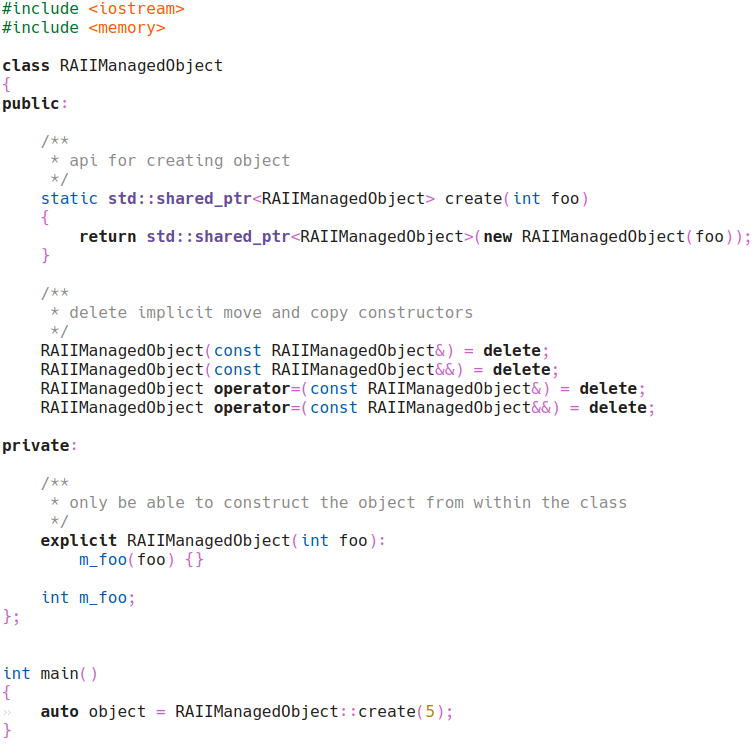
\includegraphics[width=0.7\textwidth]{obrazky-figures/raii.png}
    \caption[\textit{RAII + heap-only initialization}]{Zjednodušený pohled na \textit{RAII, heap-only initialization} filozofii. \textit{C++} má bohužel spoustu možností jak vytvořit a spravovat objekt, 
    přičemž ne každá z nich je optimální či správná. Omezení vytváření objektů v projektu unifikuje paměťovou správu a odpovědnost jednotlivých objektů.}
    \label{raii-heap-only}
\end{figure}

\section{Virtuální hardwarová komponenta}

\textit{PlayStation} ve svém hardwarovém designu připomíná velice obyčejný počítač, kterému byly odstraněny přebytečné komponenty.
\textit{Sony}, na rozdíl od svých oponentů, vytvořilo tuto konzoli z relativně dobře dokumentovaných čipů již existujících počítačů. 
Samozřejmě \textit{PlayStation} obsahuje i patentované, na míru udělané součástky, které se snaží ulehčit práci procesoru.

\begin{figure}[hbt]
    \centering
    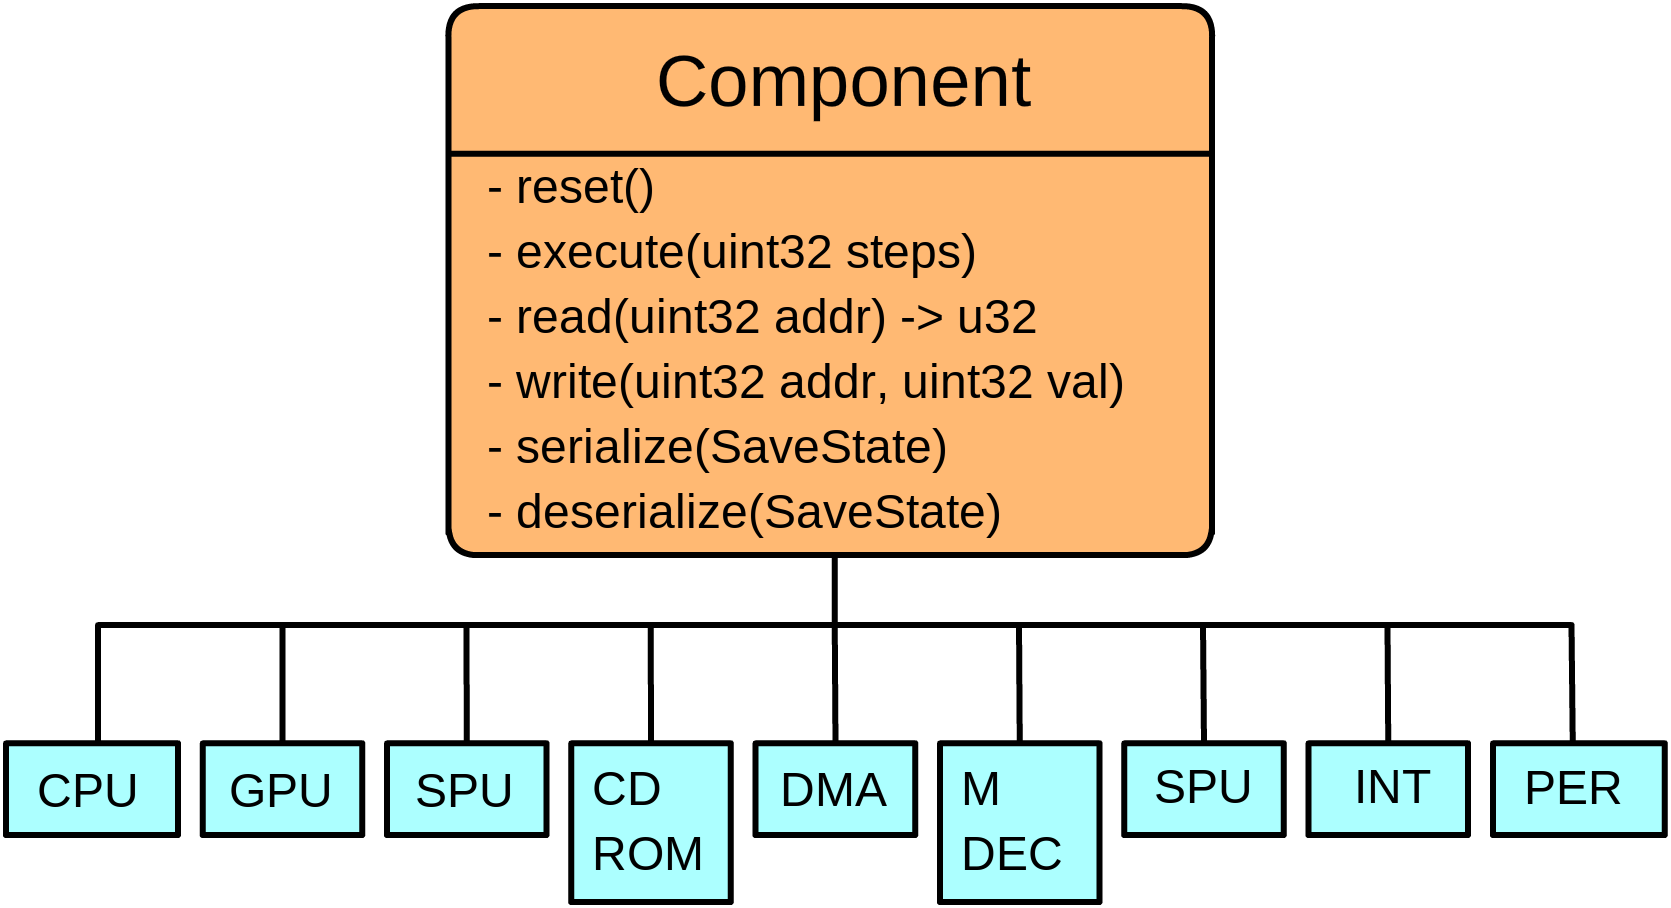
\includegraphics[width=0.6\textwidth]{obrazky-figures/component.png}
    \caption[Rozhraní hardwarové komponenty]{Rozhraní, které každá virtuální hardwarová komponenta v emulátoru musí respektovat a implementovat.}
    \label{component}
\end{figure}

Tyto hardwarové čipy sdílejí velmi podobné rozhraní. 
To je dáno tím, že interakce mezi těmito komponentami jsou založeny na \textit{Memory-mapped I/O}.
To znamená, že sběrnice systému má uniformní paměťové rozložení, přičemž jednotlivé komponenty se mapují do specifických paměťových intervalů. 
Jednotlivé komponenty pak mohou do těchto intervalů zapisovat nebo z nich číst a sběrnice pak rozdistribuuje tyto přístupy daným komponentám.
Díky tomuto faktu, v emulátoru musí mít každá virtuální hardwarová komponenta následující schopnosti:

\begin{itemize}
    \item{\textit{Reset/Inicializace}}
    \item{\textit{Čtení} z komponenty}
    \item{\textit{Zápis} do komponenty}
    \item{Provedení \textit{jednotky práce}}
    \item{\textit{Serializace}}
    \item{\textit{Deserializace}}
\end{itemize}

Pomocí dědičnosti a virtuálních metod v \textit{C++} můžeme specifikovat virtuální třídu, která bude sloužit jako základ pro všechny hlavní hardwarové komponenty, viz obrázek \ref{component}.

\section{Ukládání stavu emulátoru}

Aby se emulátor snadněji debugoval, bylo nutné vytvořit systém ukládání a načítání stavu emulátoru na disk.
Díky tomu se dají přeskočit sáhodlouhé inicializační rutiny a úvody v testovaných hrách.
Každá komponenta se tedy musí umět převést na sérii bytů a z těchto samých bytů se znovu zrekonstruovat.

Tuto zodpovědnost přebírá objekt \textit{SaveState}, který dokáže serializovat/deserializovat všechny primitiva
jednotlivých komponent.
Emulátor při ukládání/načítání svého stavu tento objekt stromovitě předá postupně všem komponentám. Jednotlivé komponenty vloží svoje atomy do \textit{SaveState} objektu při serializaci,
nebo je načtou v předem daném pořadí při deserializaci.

\section{Návrh architektury}

\textit{PlayStation} se skládá z několika hlavních hardwarových komponent. Patří sem \cite{PSXSpec}:

\begin{itemize}
    \item Sběrnice
    \item Central Processing Unit \textbf{(CPU)}
    \item Graphics Processing Unit \textbf{(GPU)}
    \item Sound Processing Unit \textbf{(SPU)}
    \item 3 Časovače/Hodiny
    \item Ovladač přerušení
    \item Ovladač přímého přístupu do paměti \textbf{(DMA)}
    \item Dekodér makrobloku \textbf{(MDEC)}
    \item CD-ROM
\end{itemize}

Každá z těchto komponent je klíčová pro správné fungování emulátoru jako celku. Zjednodušený návrh propojení je popsán
v následujícím obrázku \ref{psx-layout}, přičemž detailní návrh komponent, schopností a s kým mohou komunikovat je pak popsán v obrázku \ref{psx-layout-detailed}.

V návrhu jsou také zohledněny podřadné komponenty, které nemohou fungovat samostatně.
To se týká například komponenty \textit{Geometry Transformation Engine (GTE)}, což je
koprocesor specializující se na práci s lineární algebrou. Jelikož k této komponentě lze přistoupit
pouze skrz \textit{CPU} pomocí speciální instrukce, nelze tuto komponentu chápat jako samostatný celek.

Každá komponenta je následně propojena se sběrnicí kvůli \textit{Memory-mapped I/O}. Existují
však i přímá propojení bez sběrnice jako prostředníka. To je hlavně díky \textit{DMA} komponentě,
která zajišťuje rychlý přenos dat, aniž by se \textit{CPU} muselo o tento přenos starat. Další
přímá propojení jsou určena pro správu přerušení. Vzhledem k tomu, že přerušení může nastat skoro v
každé komponentě, je nutné toto přerušení přenášet do \textit{Ovladače výjimek}, který následně
upraví stav \textit{CPU} a přerušení se zpracuje jako výjimka.